\documentclass[11pt]{beamer}
\usetheme{Boadilla}

\usepackage{agda}
\usepackage{bbm}
\usepackage{animate}
\usepackage{hyperref}
\usepackage{graphicx}
\usepackage{longtable}
\usepackage{amsmath}
\usepackage{mdwlist}
\usepackage{txfonts}
\usepackage{xspace}
\usepackage{amstext}
\usepackage{amssymb}
\usepackage{stmaryrd}
\usepackage{proof}
\usepackage{multicol}
\usepackage[nodayofweek]{datetime}
\usepackage{etex}
\usepackage{textgreek}
\usepackage[all, cmtip]{xy}

\newcommand{\red}[1]{{\color{red}{#1}}}
\newcommand{\blue}[1]{{\color{blue}{#1}}}

\newenvironment{floatrule}
    {\hrule width \hsize height .33pt \vspace{.5pc}}
    {\par\addvspace{.5pc}}

\title{An Introduction to \\
Homotopy Type Theory}
\author{Amr Sabry}
\institute{
  School of Informatics and Computing \\
  Indiana University
}

\date{October 31, 2013} 

\begin{document}

\maketitle

\AgdaHide{
\begin{code}\>\<%
\\
\>\AgdaComment{-- \{-\# OPTIONS --without-K \#-\}}\<%
\\
\>\AgdaKeyword{module} \AgdaModule{talk1} \AgdaKeyword{where}\<%
\\
\>\AgdaKeyword{import} \AgdaModule{Level}\<%
\\
\>\AgdaKeyword{infixr} \AgdaNumber{5} \_∷\_\<%
\\
\>\AgdaKeyword{infixl} \AgdaNumber{6} \_+\_ \<%
\\
\>\AgdaKeyword{infixl} \AgdaNumber{7} \_*\_ \<%
\\
\>\<\end{code}
}

%%%%%%%%%%%%%%%%%%%%%%%%%%%%%%%%%%%%%%%%%%%%%%%%%%%%%%%%%%%%%%%%%%%%%%%%%
\begin{frame}[fragile]

\begin{center}
\scalebox{0.5}{
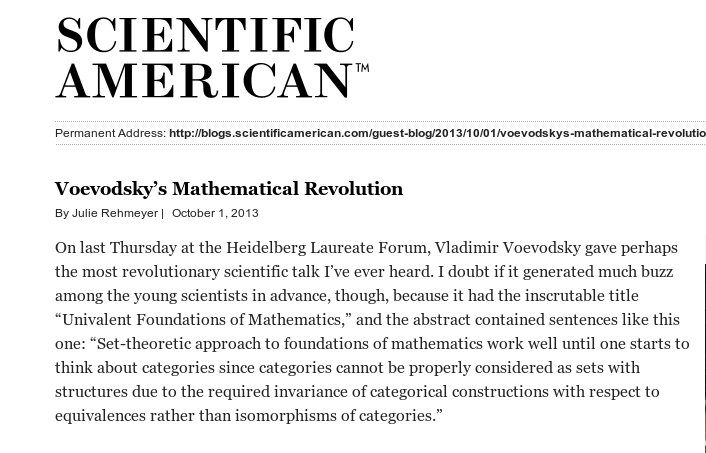
\includegraphics{pics/scientific-american.png}
}
\end{center}

\end{frame}

%%%%%%%%%%%%%%%%%%%%%%%%%%%%%%%%%%%%%%%%%%%%%%%%%%%%%%%%%%%%%%%%%%%%%%%%%
\begin{frame}{Homotopy Type Theory (HoTT)}

\begin{itemize}
\vfill\item Foundational;

\vfill\item New perspectives on old problems;

\vfill\item Connections to computer science, logic, algebra, geometry,
topology, and physics;

\vfill\item Bridges between communities;

\vfill\item What is it about exactly?

\end{itemize}

\vfill
\end{frame}

%%%%%%%%%%%%%%%%%%%%%%%%%%%%%%%%%%%%%%%%%%%%%%%%%%%%%%%%%%%%%%%%%%%%%%%%%
\begin{frame}{Steve Awodey's introduction (Feb. 2012)}

\begin{center}
\scalebox{0.9}{
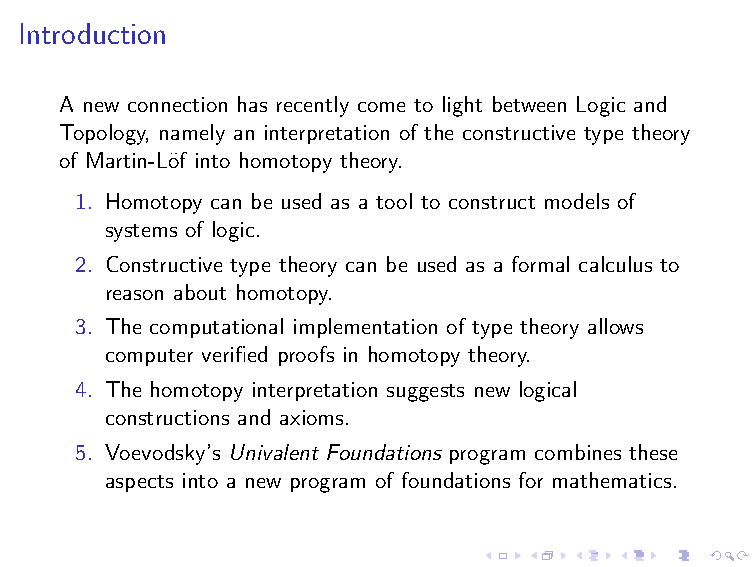
\includegraphics{pics/awodey.pdf}
}
\end{center}

\end{frame}

%%%%%%%%%%%%%%%%%%%%%%%%%%%%%%%%%%%%%%%%%%%%%%%%%%%%%%%%%%%%%%%%%%%%%%%%%
\begin{frame}{In English (bigger informal picture)}
\vfill
\begin{itemize}
\vfill\item We are discovering that \red{every} process around us has
computational content (even the design of outlines of 18th century string
instruments as developed in \blue{Functional geometry and the Trait\'e de
  Lutherie}, ICFP 2013)

\vfill\item We have known for quite a while (by the Curry-Howard
correspondence) that \red{mathematical proofs have computational content}
(\blue{type theory}, \blue{mechanized logic}, \blue{computational logic},
etc. are all well-established)

\vfill\item Feynman, Minsky, Landauer, Fredkin, and others have pushed the
thesis that \red{physical laws have computational content}. Here is one of my
favorite quotes:
\begin{quote}
  \ldots the real world is unlikely to supply us with unlimited memory or
  unlimited Turing machine tapes. Therefore, continuum mathematics is not
  executable, and physical laws which invoke that can not really be
  satisfactory \ldots
\end{quote}

\end{itemize}
\vfill
\end{frame}

%%%%%%%%%%%%%%%%%%%%%%%%%%%%%%%%%%%%%%%%%%%%%%%%%%%%%%%%%%%%%%%%%%%%%%%%%
\begin{frame}{Common Themes: Physics perspective}

\begin{itemize}

\vfill\item From the physical perspective: the laws of conservation of energy
and information translate to ``laws'' requiring computation to \red{preserve
  resources}. 

\vfill\item Linear logic is a step in that direction but more generally one
might argue that Computer Science is all about managing resources.

\vfill\item The natural way of expressing computations that preserve
resources is via \red{type isomorphisms}.

\end{itemize}
\vfill
\end{frame}

%%%%%%%%%%%%%%%%%%%%%%%%%%%%%%%%%%%%%%%%%%%%%%%%%%%%%%%%%%%%%%%%%%%%%%%%%
\begin{frame}{Common Themes: Mathematics perspective}

\begin{itemize}

\vfill\item From the mathematical side: it is important to understand the
computational content of \blue{propositional equality} $\equiv$ as opposed to
\blue{definitional equality} $=$.

\vfill\item If we claim that we have a proof that the proposition $x \equiv
y$ is true, then it is interesting to be able to produce at least one such
proof and to understand how various proofs might be connected.

\vfill\item The natural way of expressing proofs of propositional equality is
again via \red{isomorphisms between propositions}, which by the Curry-Howard
correspondence is the same as \red{type isomorphisms}.

\end{itemize}
\vfill
\end{frame}

%%%%%%%%%%%%%%%%%%%%%%%%%%%%%%%%%%%%%%%%%%%%%%%%%%%%%%%%%%%%%%%%%%%%%%%%%
\begin{frame}{HoTT, informally}
\vfill

\begin{center}

``Mathematics or Type Theory or Computation etc. with \\ 
  \ \\
  all equalities replaced by isomorphisms, \\ 
  \ \\
  i.e., with equalities given computational content.''

\end{center}

\vfill
\end{frame}

%%%%%%%%%%%%%%%%%%%%%%%%%%%%%%%%%%%%%%%%%%%%%%%%%%%%%%%%%%%%%%%%%%%%%%%%%
\begin{frame}{Isomorphisms}

\begin{itemize}
\vfill\item When are two structures isomorphic?

\vfill\item Example: are these two graphs isomorphic?

\begin{center}
\scalebox{0.3}{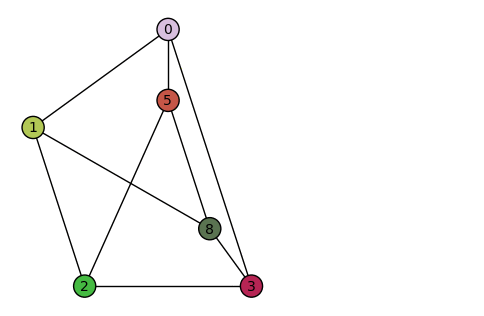
\includegraphics{pics/i-60.png}}
\scalebox{0.3}{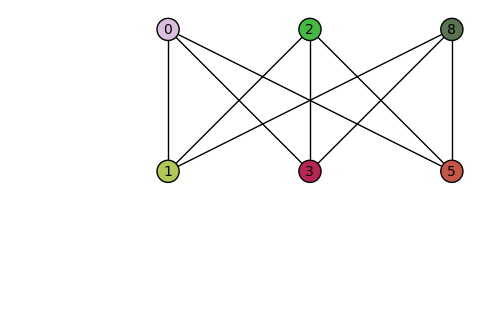
\includegraphics{pics/i-72.png}}
\end{center}

\end{itemize}

\vfill\footnotesize{In general, you don't have nice colors and numbers to
tell you which nodes correspond to which nodes.}

\end{frame}

%%%%%%%%%%%%%%%%%%%%%%%%%%%%%%%%%%%%%%%%%%%%%%%%%%%%%%%%%%%%%%%%%%%%%%%%%
\begin{frame}{Isomorphisms}

\vfill

Here is the proof that these two graphs are isomorphic.

\begin{center}
\scalebox{0.3}{\animategraphics[controls]{3}{pics/i-}{60}{72}}
\scalebox{0.3}{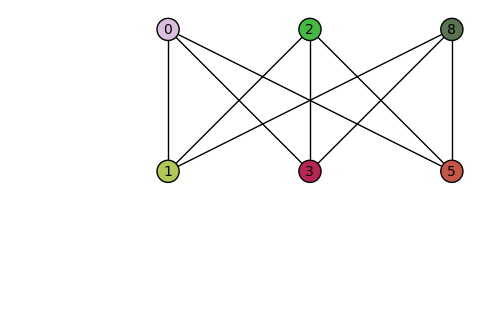
\includegraphics{pics/i-72.png}}
\end{center}

\vfill\footnotesize{[Credit to Pablo Angulo, using Sage software
    \url{http://commons.wikimedia.org/wiki/File:Kuratowski.gif}]}
\end{frame}

%%%%%%%%%%%%%%%%%%%%%%%%%%%%%%%%%%%%%%%%%%%%%%%%%%%%%%%%%%%%%%%%%%%%%%%%%
\begin{frame}{Isomorphisms}
\vfill

Two structures are isomorphic if we can \blue{morph} one to the
other by:
\begin{itemize}
\vfill\item \blue{bending},
\vfill\item \blue{shrinking}, and
\vfill\item \blue{expanding}.
\vfill\item \red{No cutting; no gluing}
\vfill\item Formally, a \red{homotopy}.
\end{itemize}
\vfill
\end{frame}

%%%%%%%%%%%%%%%%%%%%%%%%%%%%%%%%%%%%%%%%%%%%%%%%%%%%%%%%%%%%%%%%%%%%%%%%%
\begin{frame}{Homotopy}
\vfill
\begin{itemize}

\vfill\item Given two continuous functions from one topological space to
another, a homotopy is a deformation of one function into the other.

\vfill\item In homotopy type theory, we think of $x \equiv y$ as a \red{path}
from point $x$ to point $y$.

\vfill\item Different proofs lead to different paths. 

\vfill\item A homotopy is a 2-path (a path between paths) that deforms one
path to the other:
\begin{center}
\scalebox{0.5}{\animategraphics[controls]{10}{pics/Homotopy-}{0}{50}}
\end{center}

\end{itemize}

\vfill\footnotesize{[Credit: Wikipedia
    \url{http://en.wikipedia.org/wiki/Homotopy}.]}
\end{frame}

%%%%%%%%%%%%%%%%%%%%%%%%%%%%%%%%%%%%%%%%%%%%%%%%%%%%%%%%%%%%%%%%%%%%%%%%%
\begin{frame}{Mugs and donuts}

\begin{itemize}
\vfill\item No talk that mentions topology can be complete without the
obligatory coffee mug and donut.

\vfill\item This is a homotopy of one space into another:
\begin{center}
\scalebox{0.5}{\animategraphics[controls]{10}{pics/Mug-}{0}{57}}
\end{center}

\end{itemize}

\vfill\footnotesize{[Credit: Wikipedia
    \url{http://en.wikipedia.org/wiki/Homotopy}.]}
\end{frame}

%%%%%%%%%%%%%%%%%%%%%%%%%%%%%%%%%%%%%%%%%%%%%%%%%%%%%%%%%%%%%%%%%%%%%%%%%
\begin{frame}{Applications to Concurrency Theory}

\begin{itemize}

\vfill\item Different computation schedules correspond to different
\red{paths}.

\vfill\item A homotopy between two paths means that the two corresponding
schedules produce the same answers.

\vfill\item Critical regions correspond to \red{forbidden} regions. A
\red{continuous} deformation of paths \red{cannot} cross the forbidden
region:

\begin{center}
\scalebox{0.15}{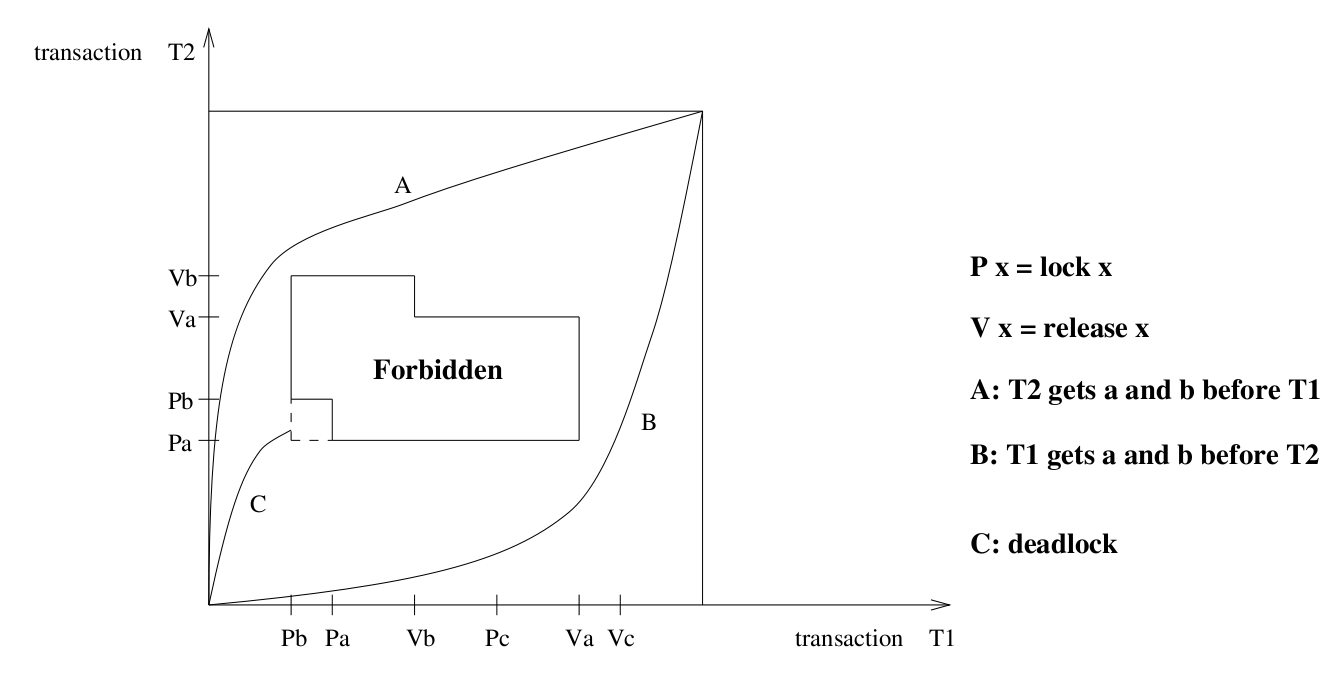
\includegraphics{pics/conc.png}}
\end{center}

\vfill\item The schedules on each side of the forbidden region might lead to
different observable answers.

\end{itemize}

\vfill\footnotesize{[Credit: Algebraic Topology and Concurrency, Fajstrup,
    Goubault, and Raussen, TCS 1998]}
\end{frame}

%%%%%%%%%%%%%%%%%%%%%%%%%%%%%%%%%%%%%%%%%%%%%%%%%%%%%%%%%%%%%%%%%%%%%%%%%
\begin{frame}{HoTT, a bit more formally}

\begin{itemize}
\vfill\item (Martin-L\"of) type theory
\vfill\item Interpret types as topological spaces (or weak $\infty$-groupoids)
\vfill\item Interpret identities as paths
\end{itemize}

\vfill
\end{frame}

%%%%%%%%%%%%%%%%%%%%%%%%%%%%%%%%%%%%%%%%%%%%%%%%%%%%%%%%%%%%%%%%%%%%%%%%%
\begin{frame}{Martin-L\"of type theory}

\vfill
\begin{center}
Universes $+$ \\
\  \\
Dependent functions $+$ \\
\  \\
Inductive data types \\
\  \\
\uncover<2->{\red{in an executable framework}. [We use Agda for this talk.]}
\end{center}
\end{frame}

%%%%%%%%%%%%%%%%%%%%%%%%%%%%%%%%%%%%%%%%%%%%%%%%%%%%%%%%%%%%%%%%%%%%%%%%%
\begin{frame}{Basic inductive types} 

\begin{code}\>\<%
\\
\>\AgdaComment{-- the empty type; the proposition FALSE}\<%
\\
\>\AgdaKeyword{data} \AgdaDatatype{⊥} \AgdaSymbol{:} \AgdaPrimitiveType{Set} \AgdaKeyword{where} \<[19]%
\>[19]\<%
\\
%
\\
\>\AgdaComment{-- the type with one element}\<%
\\
\>\AgdaKeyword{data} \AgdaDatatype{⊤} \AgdaSymbol{:} \AgdaPrimitiveType{Set} \AgdaKeyword{where}\<%
\\
\>[0]\AgdaIndent{2}{}\<[2]%
\>[2]\AgdaInductiveConstructor{tt} \AgdaSymbol{:} \AgdaDatatype{⊤}\<%
\\
%
\\
\>\AgdaKeyword{data} \AgdaDatatype{Bool} \AgdaSymbol{:} \AgdaPrimitiveType{Set} \AgdaKeyword{where}\<%
\\
\>[0]\AgdaIndent{2}{}\<[2]%
\>[2]\AgdaInductiveConstructor{false} \<[9]%
\>[9]\AgdaSymbol{:} \AgdaDatatype{Bool}\<%
\\
\>[0]\AgdaIndent{2}{}\<[2]%
\>[2]\AgdaInductiveConstructor{true} \<[9]%
\>[9]\AgdaSymbol{:} \AgdaDatatype{Bool}\<%
\\
\>\<\end{code}
\end{frame}

%%%%%%%%%%%%%%%%%%%%%%%%%%%%%%%%%%%%%%%%%%%%%%%%%%%%%%%%%%%%%%%%%%%%%%%%%
\begin{frame}{Basic inductive types (ctd.)}

\begin{code}\>\<%
\\
\>\AgdaKeyword{data} \AgdaDatatype{ℕ} \AgdaSymbol{:} \AgdaPrimitiveType{Set} \AgdaKeyword{where}\<%
\\
\>[0]\AgdaIndent{2}{}\<[2]%
\>[2]\AgdaInductiveConstructor{zero} \<[8]%
\>[8]\AgdaSymbol{:} \AgdaDatatype{ℕ}\<%
\\
\>[0]\AgdaIndent{2}{}\<[2]%
\>[2]\AgdaInductiveConstructor{suc} \<[8]%
\>[8]\AgdaSymbol{:} \AgdaDatatype{ℕ} \AgdaSymbol{→} \AgdaDatatype{ℕ}\<%
\\
%
\\
\>\AgdaComment{-- disjoint unions or coproducts}\<%
\\
\>\AgdaKeyword{data} \AgdaDatatype{\_⊎\_} \AgdaSymbol{(}\AgdaBound{A} \AgdaBound{B} \AgdaSymbol{:} \AgdaPrimitiveType{Set}\AgdaSymbol{)} \AgdaSymbol{:} \AgdaPrimitiveType{Set} \AgdaKeyword{where}\<%
\\
\>[0]\AgdaIndent{2}{}\<[2]%
\>[2]\AgdaInductiveConstructor{inj₁} \AgdaSymbol{:} \AgdaBound{A} \AgdaSymbol{→} \AgdaBound{A} \AgdaDatatype{⊎} \AgdaBound{B}\<%
\\
\>[0]\AgdaIndent{2}{}\<[2]%
\>[2]\AgdaInductiveConstructor{inj₂} \AgdaSymbol{:} \AgdaBound{B} \AgdaSymbol{→} \AgdaBound{A} \AgdaDatatype{⊎} \AgdaBound{B}\<%
\\
\>\<\end{code}
\AgdaHide{
\begin{code}\>\<%
\\
\>\AgdaSymbol{\{-\#} \AgdaKeyword{BUILTIN} NATURAL \AgdaDatatype{ℕ} \AgdaSymbol{\#-\}}\<%
\\
\>\AgdaSymbol{\{-\#} \AgdaKeyword{BUILTIN} ZERO \AgdaInductiveConstructor{zero} \AgdaSymbol{\#-\}}\<%
\\
\>\AgdaSymbol{\{-\#} \AgdaKeyword{BUILTIN} SUC \AgdaInductiveConstructor{suc} \AgdaSymbol{\#-\}}\<%
\\
\>\<\end{code}
}
\begin{code}\>\<%
\\
\>\AgdaFunction{nb₁} \AgdaSymbol{:} \AgdaDatatype{ℕ} \AgdaDatatype{⊎} \AgdaDatatype{Bool}\<%
\\
\>\AgdaFunction{nb₁} \AgdaSymbol{=} \AgdaInductiveConstructor{inj₁} \AgdaNumber{3}\<%
\\
%
\\
\>\AgdaFunction{nb₂} \AgdaSymbol{:} \AgdaDatatype{ℕ} \AgdaDatatype{⊎} \AgdaDatatype{Bool}\<%
\\
\>\AgdaFunction{nb₂} \AgdaSymbol{=} \AgdaInductiveConstructor{inj₂} \AgdaInductiveConstructor{true}\<%
\\
\>\<\end{code}

\end{frame}

%%%%%%%%%%%%%%%%%%%%%%%%%%%%%%%%%%%%%%%%%%%%%%%%%%%%%%%%%%%%%%%%%%%%%%%%%
\begin{frame}{Universes} 

\begin{itemize}
\vfill\item A \red{universe} is a ``set'' whose elements are ``sets''.
\vfill\item A \red{universe} is a ``type'' whose elements are ``types''.
\vfill\item There is no set of all sets, obviously.
\vfill\item There is a \blue{hierarchy} of universes
\end{itemize}
\vfill
\end{frame}

%%%%%%%%%%%%%%%%%%%%%%%%%%%%%%%%%%%%%%%%%%%%%%%%%%%%%%%%%%%%%%%%%%%%%%%%%
\begin{frame}{Universes (ctd.)} 

\begin{code}\>\<%
\\
\>\AgdaFunction{n} \AgdaSymbol{:} \AgdaDatatype{ℕ}\<%
\\
\>\AgdaFunction{n} \AgdaSymbol{=} \AgdaNumber{5}\<%
\\
%
\\
\>\AgdaFunction{t} \AgdaSymbol{:} \AgdaPrimitiveType{Set₀} \AgdaComment{-- or just Set}\<%
\\
\>\AgdaFunction{t} \AgdaSymbol{=} \AgdaDatatype{ℕ}\<%
\\
%
\\
\>\AgdaFunction{t'} \AgdaSymbol{:} \AgdaPrimitiveType{Set₁}\<%
\\
\>\AgdaFunction{t'} \AgdaSymbol{=} \AgdaPrimitiveType{Set₀}\<%
\\
%
\\
\>\AgdaFunction{t''} \AgdaSymbol{:} \AgdaPrimitiveType{Set₂}\<%
\\
\>\AgdaFunction{t''} \AgdaSymbol{=} \AgdaPrimitiveType{Set₁}\<%
\\
\>\<\end{code}

\end{frame}

%%%%%%%%%%%%%%%%%%%%%%%%%%%%%%%%%%%%%%%%%%%%%%%%%%%%%%%%%%%%%%%%%%%%%%%%%
\begin{frame}{Universes and families of sets} 

\red{Families of sets} or \red{type families} or \red{dependent types}:

\begin{code}\>\<%
\\
\>\AgdaFunction{P} \AgdaSymbol{:} \AgdaDatatype{ℕ} \AgdaSymbol{→} \AgdaPrimitiveType{Set}\<%
\\
\>\AgdaFunction{P} \AgdaInductiveConstructor{0} \<[11]%
\>[11]\AgdaSymbol{=} \AgdaSymbol{\{!!\}}\<%
\\
\>\AgdaFunction{P} \AgdaSymbol{(}\AgdaInductiveConstructor{suc} \AgdaBound{n}\AgdaSymbol{)} \<[11]%
\>[11]\AgdaSymbol{=} \AgdaSymbol{\{!!\}}\<%
\\
%
\\
\>\AgdaKeyword{data} \AgdaDatatype{Vec} \AgdaSymbol{(}\AgdaBound{A} \AgdaSymbol{:} \AgdaPrimitiveType{Set}\AgdaSymbol{)} \AgdaSymbol{:} \AgdaDatatype{ℕ} \AgdaSymbol{→} \AgdaPrimitiveType{Set} \AgdaKeyword{where}\<%
\\
\>[0]\AgdaIndent{2}{}\<[2]%
\>[2]\AgdaInductiveConstructor{[]} \<[7]%
\>[7]\AgdaSymbol{:} \AgdaDatatype{Vec} \AgdaBound{A} \AgdaInductiveConstructor{zero}\<%
\\
\>[0]\AgdaIndent{2}{}\<[2]%
\>[2]\AgdaInductiveConstructor{\_∷\_} \<[7]%
\>[7]\AgdaSymbol{:} \AgdaSymbol{∀} \AgdaSymbol{\{}\AgdaBound{n}\AgdaSymbol{\}} \AgdaSymbol{(}\AgdaBound{x} \AgdaSymbol{:} \AgdaBound{A}\AgdaSymbol{)} \AgdaSymbol{(}\AgdaBound{xs} \AgdaSymbol{:} \AgdaDatatype{Vec} \AgdaBound{A} \AgdaBound{n}\AgdaSymbol{)} \AgdaSymbol{→} \AgdaDatatype{Vec} \AgdaBound{A} \AgdaSymbol{(}\AgdaInductiveConstructor{suc} \AgdaBound{n}\AgdaSymbol{)}\<%
\\
%
\\
\>\AgdaFunction{v₁} \AgdaSymbol{:} \AgdaDatatype{Vec} \AgdaDatatype{Bool} \AgdaNumber{3}\<%
\\
\>\AgdaFunction{v₁} \AgdaSymbol{=} \AgdaInductiveConstructor{false} \AgdaInductiveConstructor{∷} \AgdaInductiveConstructor{true} \AgdaInductiveConstructor{∷} \AgdaInductiveConstructor{false} \AgdaInductiveConstructor{∷} \AgdaInductiveConstructor{[]}\<%
\\
\>\<\end{code}

\end{frame}

%%%%%%%%%%%%%%%%%%%%%%%%%%%%%%%%%%%%%%%%%%%%%%%%%%%%%%%%%%%%%%%%%%%%%%%%%
\begin{frame}{Dependent functions} 

\AgdaHide{
\begin{code}\>\<%
\\
\>\AgdaFunction{\_+\_} \AgdaSymbol{:} \AgdaDatatype{ℕ} \AgdaSymbol{→} \AgdaDatatype{ℕ} \AgdaSymbol{→} \AgdaDatatype{ℕ}\<%
\\
\>\AgdaInductiveConstructor{zero} \<[6]%
\>[6]\AgdaFunction{+} \AgdaBound{n} \AgdaSymbol{=} \AgdaBound{n}\<%
\\
\>\AgdaInductiveConstructor{suc} \AgdaBound{m} \AgdaFunction{+} \AgdaBound{n} \AgdaSymbol{=} \AgdaInductiveConstructor{suc} \AgdaSymbol{(}\AgdaBound{m} \AgdaFunction{+} \AgdaBound{n}\AgdaSymbol{)}\<%
\\
%
\\
\>\AgdaFunction{\_*\_} \AgdaSymbol{:} \AgdaDatatype{ℕ} \AgdaSymbol{→} \AgdaDatatype{ℕ} \AgdaSymbol{→} \AgdaDatatype{ℕ}\<%
\\
\>\AgdaInductiveConstructor{zero} \<[6]%
\>[6]\AgdaFunction{*} \AgdaBound{n} \AgdaSymbol{=} \AgdaInductiveConstructor{zero}\<%
\\
\>\AgdaInductiveConstructor{suc} \AgdaBound{m} \AgdaFunction{*} \AgdaBound{n} \AgdaSymbol{=} \AgdaBound{n} \AgdaFunction{+} \AgdaBound{m} \AgdaFunction{*} \AgdaBound{n}\<%
\\
\>\<\end{code}
}

\begin{code}\>\<%
\\
\>\AgdaFunction{\_++\_} \AgdaSymbol{:} \AgdaSymbol{∀} \AgdaSymbol{\{}\AgdaBound{m} \AgdaBound{n}\AgdaSymbol{\}} \AgdaSymbol{\{}\AgdaBound{A} \AgdaSymbol{:} \AgdaPrimitiveType{Set}\AgdaSymbol{\}} \AgdaSymbol{→} \AgdaDatatype{Vec} \AgdaBound{A} \AgdaBound{m} \AgdaSymbol{→} \AgdaDatatype{Vec} \AgdaBound{A} \AgdaBound{n} \AgdaSymbol{→} \AgdaDatatype{Vec} \AgdaBound{A} \AgdaSymbol{(}\AgdaBound{m} \AgdaFunction{+} \AgdaBound{n}\AgdaSymbol{)}\<%
\\
\>\AgdaInductiveConstructor{[]} \<[10]%
\>[10]\AgdaFunction{++} \AgdaBound{ys} \AgdaSymbol{=} \AgdaBound{ys}\<%
\\
\>\AgdaSymbol{(}\AgdaBound{x} \AgdaInductiveConstructor{∷} \AgdaBound{xs}\AgdaSymbol{)} \<[10]%
\>[10]\AgdaFunction{++} \AgdaBound{ys} \AgdaSymbol{=} \AgdaBound{x} \AgdaInductiveConstructor{∷} \AgdaSymbol{(}\AgdaBound{xs} \AgdaFunction{++} \AgdaBound{ys}\AgdaSymbol{)}\<%
\\
%
\\
\>\AgdaFunction{concat} \AgdaSymbol{:} \AgdaSymbol{∀} \AgdaSymbol{\{}\AgdaBound{m} \AgdaBound{n}\AgdaSymbol{\}} \AgdaSymbol{\{}\AgdaBound{A} \AgdaSymbol{:} \AgdaPrimitiveType{Set}\AgdaSymbol{\}} \AgdaSymbol{→} \AgdaDatatype{Vec} \AgdaSymbol{(}\AgdaDatatype{Vec} \AgdaBound{A} \AgdaBound{m}\AgdaSymbol{)} \AgdaBound{n} \AgdaSymbol{→} \AgdaDatatype{Vec} \AgdaBound{A} \AgdaSymbol{(}\AgdaBound{n} \AgdaFunction{*} \AgdaBound{m}\AgdaSymbol{)}\<%
\\
\>\AgdaFunction{concat} \AgdaInductiveConstructor{[]} \<[19]%
\>[19]\AgdaSymbol{=} \AgdaInductiveConstructor{[]}\<%
\\
\>\AgdaFunction{concat} \AgdaSymbol{(}\AgdaBound{xs} \AgdaInductiveConstructor{∷} \AgdaBound{xss}\AgdaSymbol{)} \<[19]%
\>[19]\AgdaSymbol{=} \AgdaBound{xs} \AgdaFunction{++} \AgdaFunction{concat} \AgdaBound{xss}\<%
\\
%
\\
\>\AgdaFunction{c₁} \AgdaSymbol{:} \AgdaDatatype{Vec} \AgdaDatatype{Bool} \AgdaNumber{6}\<%
\\
\>\AgdaFunction{c₁} \AgdaSymbol{=} \AgdaFunction{concat} \AgdaSymbol{(} \<[15]%
\>[15]\AgdaSymbol{(}\AgdaInductiveConstructor{false} \AgdaInductiveConstructor{∷} \AgdaInductiveConstructor{false} \AgdaInductiveConstructor{∷} \AgdaInductiveConstructor{[]}\AgdaSymbol{)} \<[37]%
\>[37]\AgdaInductiveConstructor{∷} \<[39]%
\>[39]\<%
\\
\>[2]\AgdaIndent{15}{}\<[15]%
\>[15]\AgdaSymbol{(}\AgdaInductiveConstructor{true} \AgdaInductiveConstructor{∷} \AgdaInductiveConstructor{true} \AgdaInductiveConstructor{∷} \AgdaInductiveConstructor{[]}\AgdaSymbol{)} \<[37]%
\>[37]\AgdaInductiveConstructor{∷}\<%
\\
\>[2]\AgdaIndent{15}{}\<[15]%
\>[15]\AgdaSymbol{(}\AgdaInductiveConstructor{false} \AgdaInductiveConstructor{∷} \AgdaInductiveConstructor{false} \AgdaInductiveConstructor{∷} \AgdaInductiveConstructor{[]}\AgdaSymbol{)} \<[37]%
\>[37]\AgdaInductiveConstructor{∷} \AgdaInductiveConstructor{[]} \AgdaSymbol{)}\<%
\\
\>\<\end{code}

\end{frame}

%%%%%%%%%%%%%%%%%%%%%%%%%%%%%%%%%%%%%%%%%%%%%%%%%%%%%%%%%%%%%%%%%%%%%%%%%
\begin{frame}{Dependent pairs}

\begin{code}\>\<%
\\
\>\AgdaKeyword{record} \AgdaRecord{Σ} \AgdaSymbol{(}\AgdaBound{A} \AgdaSymbol{:} \AgdaPrimitiveType{Set}\AgdaSymbol{)} \AgdaSymbol{(}\AgdaBound{B} \AgdaSymbol{:} \AgdaBound{A} \AgdaSymbol{→} \AgdaPrimitiveType{Set}\AgdaSymbol{)} \AgdaSymbol{:} \AgdaPrimitiveType{Set} \AgdaKeyword{where}\<%
\\
\>[0]\AgdaIndent{2}{}\<[2]%
\>[2]\AgdaKeyword{constructor} \AgdaInductiveConstructor{\_,\_}\<%
\\
\>[0]\AgdaIndent{2}{}\<[2]%
\>[2]\AgdaKeyword{field}\<%
\\
\>[2]\AgdaIndent{4}{}\<[4]%
\>[4]\AgdaField{proj₁} \AgdaSymbol{:} \AgdaBound{A}\<%
\\
\>[2]\AgdaIndent{4}{}\<[4]%
\>[4]\AgdaField{proj₂} \AgdaSymbol{:} \AgdaBound{B} \AgdaBound{proj₁}\<%
\\
\>\<\end{code}

\AgdaHide{
\begin{code}\>\<%
\\
\>\AgdaKeyword{open} \AgdaModule{Σ} \AgdaKeyword{public}\<%
\\
\>\<\end{code}
}

\begin{code}\>\<%
\\
\>\AgdaFunction{exT} \AgdaSymbol{:} \AgdaPrimitiveType{Set}\<%
\\
\>\AgdaFunction{exT} \AgdaSymbol{=} \AgdaRecord{Σ} \AgdaDatatype{ℕ} \AgdaSymbol{(λ} \AgdaBound{n} \AgdaSymbol{→} \AgdaDatatype{Vec} \AgdaDatatype{Bool} \AgdaBound{n}\AgdaSymbol{)}\<%
\\
%
\\
\>\AgdaFunction{ex₁} \AgdaSymbol{:} \AgdaFunction{exT}\<%
\\
\>\AgdaFunction{ex₁} \AgdaSymbol{=} \AgdaSymbol{(}\AgdaNumber{3} \AgdaInductiveConstructor{,} \AgdaSymbol{(}\AgdaInductiveConstructor{false} \AgdaInductiveConstructor{∷} \AgdaInductiveConstructor{true} \AgdaInductiveConstructor{∷} \AgdaInductiveConstructor{false} \AgdaInductiveConstructor{∷} \AgdaInductiveConstructor{[]}\AgdaSymbol{))}\<%
\\
%
\\
\>\AgdaFunction{ex₂} \AgdaSymbol{:} \AgdaFunction{exT}\<%
\\
\>\AgdaFunction{ex₂} \AgdaSymbol{=} \AgdaSymbol{(}\AgdaNumber{0} \AgdaInductiveConstructor{,} \AgdaInductiveConstructor{[]}\AgdaSymbol{)}\<%
\\
\>\<\end{code}

\end{frame}

%%%%%%%%%%%%%%%%%%%%%%%%%%%%%%%%%%%%%%%%%%%%%%%%%%%%%%%%%%%%%%%%%%%%%%%%%
\begin{frame}{Pause}

\vfill
\begin{center}
\LaTeX\ crash \ldots \\
Switch to second talk
\end{center}
\vfill

\end{frame}

%%%%%%%%%%%%%%%%%%%%%%%%%%%%%%%%%%%%%%%%%%%%%%%%%%%%%%%%%%%%%%%%%%%%%%%%%
\end{document}

